\begin{frame}
  \titlepage
\end{frame}


\begin{frame}\frametitle{Gianluca Della Vedova}
\begin{itemize}
\item
Elementi di Bioinformatica
\item
Ufficio U14-2041
\item
\url{https://gianluca.dellavedova.org}
\item
\url{https://elearning.unimib.it/course/view.php?id=15423}
\item
\url{gianluca.dellavedova@unimib.it}
\item\url{https://github.com/bioinformatica-corso/programmi-elementi-bioinformatica}
\item\url{https://github.com/bioinformatica-corso/lezioni}
\end{itemize}
\end{frame}

\begin{frame}[fragile]
\frametitle{Notazione}
\begin{itemize}
\item
\alert{simbolo}: $T[i]$\\
\item
\alert{stringa}: $T[1]T[2]\cdots T[l]$\\
\item
\alert{sottostringa}: $T[i:j]$\\
\item
\alert{prefisso}: $T[:j]=T[1:j]$\\
\item
\alert{suffisso}: $T[i:]=T[i:|T|]$
\item
\alert{concatenazione}: $T_{1}\cdot T_{2} = T_{1}T_{2}$
\end{itemize}
\end{frame}


\begin{frame}[fragile]
\frametitle{Pattern Matching}
\begin{block}{Problema}
\alert{Input}: testo $T=T[1]\cdots T[n]$, pattern $P=P[1]\cdots P[m]$, alfabeto $\Sigma$\\
\alert{Goal}: trovare \emph{tutte} le occorrenze di $P$ in $T$\\
\alert{Goal}: trovare tutti gli $i$ tale che $T[i]\cdots T[i+m-1]=P$
\end{block}
\begin{block}{Algoritmo banale}
\alert{Tempo}: $O(nm)$
\end{block}
\begin{block}{Lower bound}
\alert{Tempo}: $O(n+m)$
\end{block}
\end{frame}

\begin{frame}
\frametitle{Bit-parallel}
\begin{block}{Algoritmi seminumerici}
\begin{itemize}
\item
$25$
\item
$25=00011001$
\item
$25=00011001=$FFFTTFFT
\end{itemize}
\end{block}
\begin{block}{Operazioni bit-level}
\alert{Or}: $x\lor y$, \alert{And}: $x\land y$, \alert{Xor}: $x\oplus y$\\
\alert{Left Shift}: $x << k$, \alert{Right Shift}: $x >> k$,
\begin{itemize}
\item
Tutte bitwise
\item
Tutte in hardware
\end{itemize}
\end{block}
\end{frame}

\begin{frame}
\frametitle{D\"om\"olki / Baeza-Yates, Gonnet}
\begin{block}{Matrice $M$}
$M(i,j)=1$ sse $P[:i]=T[j-i+1:j]$\\
$0\le i\le m$, $0\le j\le n$
\end{block}
\begin{block}{Occorrenza di $P$ in $T$}
$M(m,\cdot)=1$
\end{block}
\begin{itemize}
\item
$M(0,\cdot)=1$, $M(\cdot,0)=0$
\item
\alert{$M(i,j)=1$} sse $M(i-1, j-1)=1$ AND $P[i]=T[j]$
\end{itemize}
\end{frame}

\begin{frame}
\frametitle{Esempio}
\begin{block}{Esempio}
$T$=abracadabra\\
$P$=abr
\end{block}

\begin{center}
\begin{tabular}[l]{ll}
%\hline{1}
10010101001\\
01000000100\\
00100000010&$\leftarrow$ \alert{occorrenze}\\%\hline
\end{tabular}
\end{center}

\begin{block}{Matrice $M$}
1 colonna = 1 numero
\end{block}
\end{frame}

\begin{frame}[fragile]
\frametitle{Colonne}
$U[\sigma]$ = array di bit dove $U[\sigma,i]=1$ sse $P[i]=\sigma$

\begin{block}{$C[j]$ da $C[j-1]$}
\begin{itemize}
\item
Right shift di $C[j-1]$
\item
$1$ in prima posizione
\item
AND con $U[T[j]]$
\item
\alert{$\omega$}: word size
\item
$C[j] = \left( \left(C[j-1] >> 1 \right) \  | \  \left(1 << (\omega -1) \right) \right)\ \&\  U[T[j]]$;
\end{itemize}
\end{block}
\end{frame}

\begin{frame}[fragile]
\frametitle{Note}
\begin{itemize}
\item
Tempo $O(n)$ se $m\le \omega$
\item
Tempo $O(nm)$
\item
No condizioni
\item
$\omega < m\le 2\omega$?
\end{itemize}
\end{frame}

\begin{frame}[fragile]
\frametitle{Karp-Rabin}
\begin{block}{Alfabeto binario}
\begin{itemize}
\item
$H(S)=\sum_{i=1}^{|S|} 2^{|S| - i}H(S[i])$
\item
sliding window di ampiezza $m$ su $T$
\item
$H(T[i+1:i+m]) =$\\
$=\left(H(T[i:i+m-1]) - T[i] \right) / 2 + 2^{m-1}T[i+m]$
\item
operazioni su bit
\item
$T[i:i+m-1]=P \Leftrightarrow H(T[i:i+m-1])=H(P)$
\end{itemize}
\end{block}
\end{frame}

\begin{frame}[fragile]
\frametitle{Karp-Rabin: problema}
\begin{block}{Numeri troppo grandi}
\begin{itemize}
\item
Modello RAM: numeri $O(n+m)$
\item
mod $p$
\item
$H(T[i+1:i+m]) =$\\
$\left(\left(H(T[i:i+m-1]) - T[i] \right) / 2 + 2^{m-1}T[i+m] \right)\mod p$
\item \textbf{NO}
\item
$2^{m-1}T[i+m] \mod p$ calcolato iterativamente, $\mod p$ ad ogni passo
\end{itemize}
\end{block}
\end{frame}

\begin{frame}[fragile]
\frametitle{Karp-Rabin: falsi positivi}
\begin{block}{Possibili errori}
\begin{itemize}
\item
Falso positivo (FP): occorrenza non vera
\item
Falso negativo (FN): occorrenza non trovata
\item
$H(T[i:i+m-1])=H(P) \Leftrightarrow T[i:i+m-1]=P$
\item
$H(T[i:i+m-1])  \mod p = H(P)  \mod p$
$\Leftarrow T[i:i+m-1]=P$
\end{itemize}
\end{block}
\end{frame}


\begin{frame}[fragile]
\frametitle{Karp-Rabin: falsi positivi}
\begin{block}{Probabilità di errore}
$P[\#FP\ge 1] \le O(nm/I)$ se il numero primo $p$ è scelto fra tutti i primi $\le
I$
\end{block}

\begin{block}{Valori di $I$}
\begin{itemize}
\item
$I=n^{2}m \Rightarrow P[\#FP\ge 1] \le 2.54/n$
\item
$I=nm^{2}  \Rightarrow P[\#FP\ge 1] \in O(1/m)$
\end{itemize}
\end{block}

\begin{block}{Abbassare probabilità di errore}
Scegliere $k$ primi casuali (indipendenti senza ripetizioni), cambiare primo
dopo ogni FP
\end{block}
\end{frame}

\begin{frame}[fragile]
\frametitle{Las Vegas vs.
  Monte Carlo}
\begin{block}{Classificazione algoritmi probabilistici}
\begin{itemize}
\item
Las Vegas:
\begin{itemize}
\item
Sempre corretto
\item
Forse non veloce
\item
Quicksort con pivot random
\end{itemize}
\item
Monte Carlo:
\begin{itemize}
\item
Sempre veloce

\item
Forse non corretto
\item
Karp-Rabin
\end{itemize}
\end{itemize}
\end{block}
\end{frame}


\begin{frame}[fragile]
\frametitle{Controllo falsi positivi}
$L$: posizioni iniziali in $T$ delle occorrenze
\begin{block}{Run}
sequenza $\langle l_{1}, \ldots, l_{k}\rangle$ di posizioni in $L$ distanti al
massimo $m/2$
\end{block}

\begin{itemize}
\item
$d=l_{2}-l_{1}$
\item
$P$ semiperiodico con periodo $d$
\item
$P=\alpha\beta^{k-1}$, $\alpha$ suffisso di $\beta$
\item
ogni run occupa $\ge n$ caratteri di $T$
\item
ogni carattere  di $T$ è in max $2$ run
\end{itemize}
\end{frame}


\begin{frame}[fragile]
\frametitle{Trie}
\begin{columns}
\begin{column}{0.6\textwidth}
\begin{block}{Trie}
\begin{itemize}
\item
Albero
\item
Query: parola $\in$ dizionario
\item
archi etichettati
\item
Percorso radice-foglia = parola
\end{itemize}
\end{block}
\begin{block}{Dizionario}
ABRACADABRA\\
ARRAY\\
\uncover<3->{\alert{ABRA}}
\end{block}
\end{column}
\begin{column}{0.4\textwidth}
\begin{center}
\onslide<2-3>{\includegraphics[width=\textwidth]{figures/trie1}}
%\onslide<4->{\includegraphics[width=\textwidth]{figures/trie3}}
\end{center}
\end{column}
\end{columns}
\end{frame}

\begin{frame}[fragile]
\frametitle{Trie}
\begin{columns}
\begin{column}{0.6\textwidth}
\begin{block}{Terminatore}
\$ non appartiene all'alfabeto
\end{block}
\onslide<2->{\begin{block}{Dizionario}
ABRACADABRA\$\\
ARRAY\$\\
ABRA\$
\end{block}}
\end{column}
\begin{column}{0.4\textwidth}
\begin{center}
\onslide<3->{\includegraphics[width=\textwidth]{figures/trie4}}
\end{center}
\end{column}
\end{columns}
\end{frame}

\begin{frame}[fragile]
\frametitle{Suffix tree}
\begin{columns}
\begin{column}{0.5\textwidth}
\begin{block}{Definizione}
\begin{itemize}[<+->]
% \item
% Testo $T$
\item
Trie compatto di tutti i suffissi di $T\$$
\item
Le etichette degli archi uscenti da $x$ iniziano con simboli diversi
\item
suffissi $\Leftrightarrow$ percorso radice-foglia
\end{itemize}
\end{block}
\end{column}
\begin{column}{0.5\textwidth}
\begin{center}
\uncover<4->{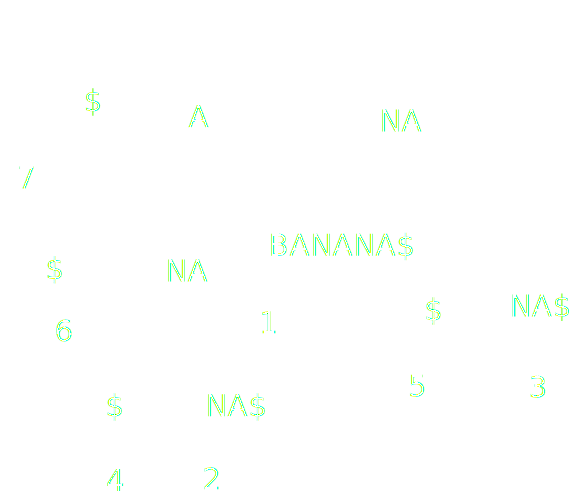
\includegraphics[width=\textwidth]{figures/Suffix_tree_BANANA}

BANANA\$}
\end{center}
\end{column}
\end{columns}
\end{frame}

\begin{frame}[fragile]
\frametitle{Suffix tree 2: Definizione}
\begin{itemize}
\item
foglie etichettata con posizione inizio suffisso
\item
path-label$(x)$: concatenazione etichette
\item
string-depth$(x)$: lunghezza path-label$(x)$
\item
Pattern matching = visita
\end{itemize}
\begin{block}{Problemi}
\begin{itemize}[<+->]
\item
Spazio $O(n^{2})$
\item
Puntatori al testo (posizioni)
\item
Spazio $20n$ bytes
\end{itemize}
\end{block}
\end{frame}

\begin{frame}[fragile]
\frametitle{Suffix array}
\begin{block}{Definizione}
\begin{itemize}[<+->]
\item
Array dei suffissi in ordine lessicografico
\item
Posizioni iniziali del suffisso nell'array
\item
Spazio $4n$ bytes
\item
$Lcp[i]$: lunghezza prefisso comune $SA[i]$, $SA[i+1]$
\end{itemize}
\end{block}
\uncover<5->{\begin{block}{BANANA\$}
\begin{tabular}[l]{|c|l|l|l|l|l|l|l|}
\hline
$i$&0&1&2&3&4&5&6\\
$SA$&7&6&4&2&1&5&3\\
$Lcp$&0&1&3&0&0&2&-\\\hline
\end{tabular}}
\end{block}
\end{frame}

\begin{frame}[fragile]
\frametitle{Da Suffix tree a Suffix array}
\begin{columns}
\begin{column}{0.5\textwidth}
\begin{itemize}[<+->]
\item
Visita depth-first di $ST$
\item
archi uscenti di ogni nodo in ordine lessicografico
\item
$Lcp[i]$ = string-depth di $lca(i,i+1)$
\end{itemize}
\end{column}
\begin{column}{0.4\textwidth}
\begin{center}
\onslide<1->{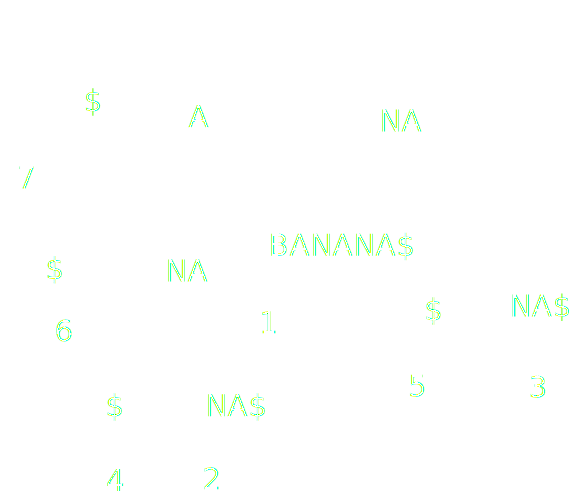
\includegraphics[width=\textwidth]{figures/Suffix_tree_BANANA}}
%\onslide<4->{\includegraphics[width=\textwidth]{figures/trie3}}
\end{center}
\end{column}
\end{columns}
\end{frame}

\begin{frame}[fragile]
\frametitle{Da Suffix array a Suffix tree}
\begin{columns}
\begin{column}{0.5\textwidth}
\begin{itemize}[<+->]
\item
$Lcp = 0$:  partizione $SA$
\item
corrispondono ai figli della radice
\item
ricorsione prendendo i numeri minimi
\end{itemize}
\begin{block}{BANANA\$}
\begin{tabular}[l]{|c|l|l|l|l|l|l|l|}
\hline
$i$&0&1&2&3&4&5&6\\
$SA$&7&6&4&2&1&5&3\\
$Lcp$&0&1&3&0&0&2&-\\\hline
\end{tabular}
\end{block}
\end{column}
\begin{column}{0.5\textwidth}
\begin{center}
\only<2>{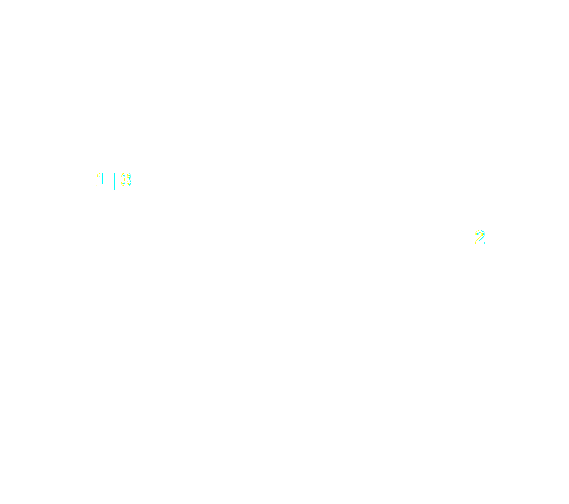
\includegraphics[width=\textwidth]{figures/Suffix_tree_BANANA-level1}}
\only<3>{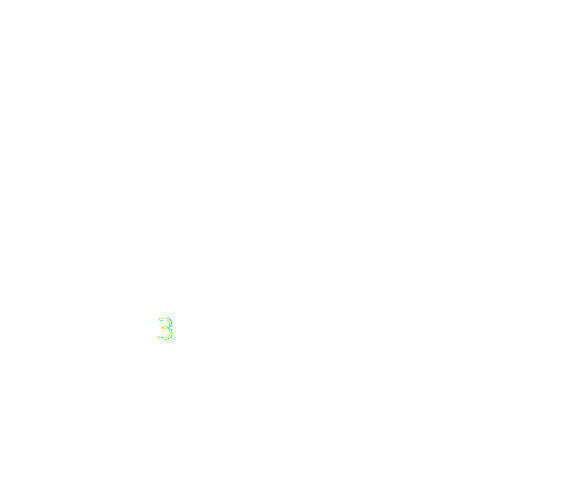
\includegraphics[width=\textwidth]{figures/Suffix_tree_BANANA-level2}}
\only<4>{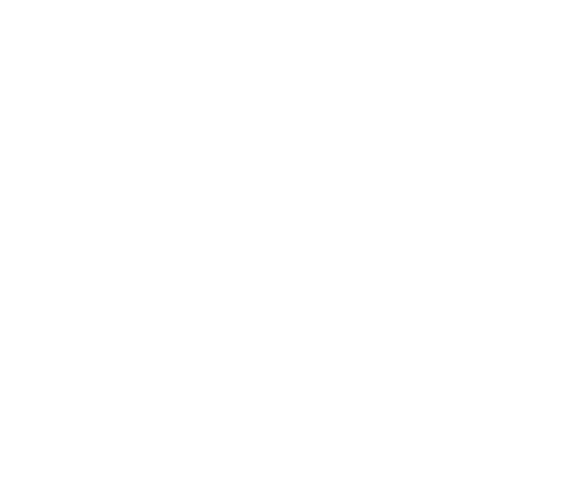
\includegraphics[width=\textwidth]{figures/Suffix_tree_BANANA-level3}}
\only<5>{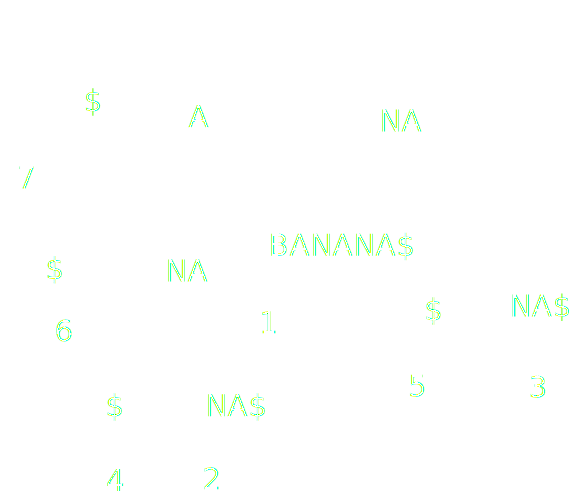
\includegraphics[width=\textwidth]{figures/Suffix_tree_BANANA}}
\end{center}
\end{column}
\end{columns}
\end{frame}

\begin{frame}[fragile]
\frametitle{Sottostringa comune più lunga di due stringhe}
\begin{block}{Due stringhe $s_{1}$ e $s_{2}$}
\begin{itemize}[<+->]
\item
Suffix tree generalizzato = insieme di stringhe
\item
$ST(s_{1}\$_{1}s_{2}\$_{2})$
\item
Nodo $x$ con foglie di $s_{1}$ e $s_{2}$
\item
Sottostringa di $s_{1}$ e $s_{2}$
\item
$ST(s_{1}\$s_{2}\$)$
\item
Max string-depth
\end{itemize}
\end{block}
\end{frame}



\begin{frame}
\frametitle{Suffix tree generalizzato}
\begin{center}
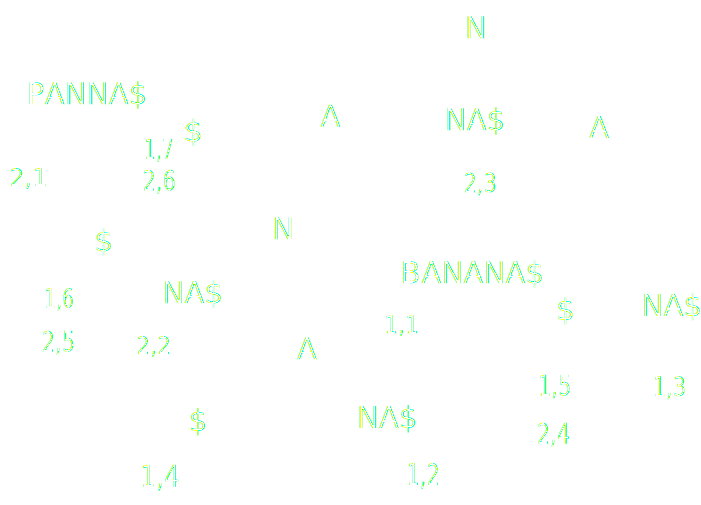
\includegraphics[width=0.8\textwidth]{figures/ST-banana-panna}
\end{center}
$s_{1}$: BANANA\$, $s_{2}$: PANNA\$
\end{frame}


\begin{frame}[fragile]
\frametitle{Pattern matching su suffix array}
\begin{block}{Occorrenza $P$ in $T$}
Suffissi di $T$ che iniziano con $P$
\end{block}
\begin{block}{Ricerca in $SA$}
\begin{itemize}
\item
Ricerca dicotomica
\item
Tempo $O(m \log n)$ -- caso pessimo
\item
Controllare tutto $P$ ad ogni iterazione
\item
$log_{2} n$ iterazioni
\end{itemize}
\end{block}
\end{frame}

\begin{frame}[fragile]
\frametitle{Acceleranti 1}
\begin{columns}
\begin{column}{0.5\textwidth}
\begin{itemize}
\item
Intervallo $SA(L, R)$ di $SA$
\item
Elemento mediano $M$
\item
Tutti i suffissi in $SA(L,R)$ iniziano con uno stesso prefisso lungo $Lcp(SA[L],
SA[R])$
\item
Non confrontare con i primi $Lcp(SA[L], SA[R])$ caratteri
\end{itemize}
\end{column}
\begin{column}{0.4\textwidth}
\begin{center}
\onslide<1->{\multiinclude[<+>][start=1,format=pdf,graphics={width=0.95\textwidth}]{figures/SA-pattern-matching1}}
%\onslide<4->{\includegraphics[width=\textwidth]{figures/trie3}}
\end{center}
\end{column}
\end{columns}
\end{frame}

\begin{frame}[fragile]
\frametitle{Acceleranti 2}
\begin{columns}[T]
\begin{column}[T]{0.6\textwidth}
\begin{block}{$l$: $lcp(L,P)$; $r$: $Lcp(R,P)$}
\begin{enumerate}
\item
Caso 1: $l>r$
\only<3->{\begin{itemize}\item
$Lcp(L,M)>l$\only<4->{$\Rightarrow L\gets M$}
\only<5->{\item
$Lcp(L,M)<l$\only<6->{$\Rightarrow$\\ $R\gets M, r\gets Lcp(M,L)$}}
\only<7->{\item
  $Lcp(L,M)=l$\only<8->{$\Rightarrow$ confronto $P[l+1:]$, $M[l+1:]$}
}\end{itemize}}
\only<9->{\item
  Caso 2: $l=r$
\only<10->{\begin{itemize}\item
  $Lcp(L,M)>l$
\only<11->{\item $Lcp(M,R)>l$}
\only<12->{\item $Lcp(L,M)=Lcp(M,R)=l$}
  \end{itemize}}}
\end{enumerate}
\end{block}
\end{column}
\begin{column}{0.38\textwidth}
\only<2->{\multiinclude[<+>][start=1,format=pdf,graphics={width=0.95\textwidth}]{figures/SA-accelerant}}
%\only<2->{\multiinclude[<alert@+| +->][start=1,format=pdf,graphics={width=0.95\textwidth}]{figures/SA-accelerant}}
\end{column}
\end{columns}
\end{frame}

\begin{frame}[fragile]
\frametitle{Acceleranti 2: calcolo $Lcp$ in tempo $O(n)$}
\begin{itemize}[<+->]
\item
Iterazione 1: $(L,R)=(1,m)$
\item
Iterazione 2: $(L,R)=(1,m/2)$ oppure $(m/2,m)$
\item
Iterazione $k$: $L = h\frac{m}{2^{k-1}}$, $R = (h+1)\frac{m}{2^{k-1}}$
\item
Iterazione $\lceil \log_{2}m\rceil$: $R=L+1$, $Lcp(h,h+1)$
\item
Iterazione $\lceil \log_{2}m\rceil -1$: aggrego i risultati dell'iterazione
$\lceil \log_{2}m\rceil$
\item
Iterazione $k$: $Lcp(h\frac{m}{2^{k-1}}, (h+1)\frac{m}{2^{k-1}})$
\item
$=\min\{Lcp(2h\frac{m}{2^{k}}, (2h+1)\frac{m}{2^{k}})$,
$Lcp((2h+1)\frac{m}{2^{k}}+1, (2h+2)\frac{m}{2^{k}})$,
$Lcp((2h+1)\frac{m}{2^{k}}), Lcp((2h+1)\frac{m}{2^{k}}+1)\}$
\end{itemize}
\end{frame}


\begin{frame}[fragile]
\frametitle{Acceleranti 2: calcolo $Lcp$ in tempo $O(n)$}
\multiinclude[<+>][start=1,format=pdf,graphics={width=0.95\textwidth}]{figures/SA-linear-Lcp}
\uncover<5->{Passaggio da $y$ a $z$ deve esistere}
\end{frame}

\begin{frame}
\frametitle{Acceleranti 2: Osservazione}
\begin{itemize}[<+->]
\item
Tempo per trovare un'occorrenza
\item
Tempo per trovare tutte le occorrenze?
\item
$O(n+m+k)$, per $k$ occorrenze
\end{itemize}
\end{frame}

\begin{frame}
\frametitle{Costruzione suffix array: nuovo alfabeto}
\begin{itemize}
\item
Alfabeto $\Sigma$ con $\sigma$ simboli, testo $T$ lungo $n$
\item
Aggrego triple di caratteri
\item
Alfabeto $\Sigma^{3}$ con $\sigma^{3}$ simboli, testo lungo $n/3$
\item
$T_{1}=(T[1],T[2],T[3])\cdots (T[3i+1],T[3i+2],T[3i+3])\cdots$\\
$T_{2}=(T[2],T[3],T[4])\cdots (T[3i+2],T[3i+3],T[3i+4])\cdots$\\
$T_{0}=(T[3],T[4],T[5])\cdots (T[3i],T[3i+1],T[3i+2])\cdots$
\item
suffissi$(T)$ $\Leftrightarrow$ $\bigcup_{i=0,1,2}$ suffissi$(T_{i})$
\end{itemize}
\end{frame}

\begin{frame}
\frametitle{Costruzione suffix array: ricorsione}
\begin{enumerate}
\item
Ricorsione su $T_{0}T_{1}$
\item
suffissi$(T_{0}T_{1})$ $\Leftrightarrow$ suffissi$(T_{0})$, suffissi$(T_{1})$
\item
suffissi$(T_{0}T_{1})$  $\Leftrightarrow$ suffissi$(T_{2})$
\item
$T_{2}[i:] \approx T[3i+2:]$
\item
$T[3i+2:] = T[3i+2]T[3i+3:] =T[3i+2]T_{0}[i+1:]$
\item
suffissi$(T_{0})$ ordinati
\item
Radix sort
\item
Fusione suffissi$(T_{0}T_{1})$,  suffissi$(T_{2})$
\end{enumerate}
\end{frame}

\begin{frame}
\frametitle{Costruzione suffix array: fusione}
Confronto suffisso di $T_{0}$ e $T_{2}$
\begin{enumerate}
\item
$T_{0}[i:] <=> T_{2}[j:]$
\item
$T[3i:] <=> T[3j+2:]$
\item
$T[3i]T[3i+1:] <=> T[3j+2]T[3j+3:]$
\item
$T[3i]T_{1}[i:] <=> T[3j+2]T_{0}[j+1:]$
\end{enumerate}
\end{frame}



\begin{frame}
\frametitle{Costruzione suffix array: fusione}
Confronto suffisso di $T_{1}$ e $T_{2}$
\begin{enumerate}
\item
$T_{1}[i:] <=> T_{2}[j:]$
\item
$T[3i+1:] <=> T[3j+2:]$
\item
$T[3i+1]T[3i+2:] <=> T[3j+2]T[3j+3:]$
\item
$T[3i+1]T[3i+2]T[3i+3:] <=> T[3j+2]T[3j+3]T[3j+4:]$
\item
$T[3i+1]T[3i+2]T_{0}[i+1:] <=> T[3j+2]T[3j+3]T_{1}[j+1:]$
\end{enumerate}
\end{frame}

\begin{frame}
\frametitle{KS}
\begin{enumerate}
\item
Juha Kärkkäinen, Peter Sanders and Stefan Burkhardt.
Linear work suffix array construction. J. ACM, 53 (6), 2006, pp. 918-936.
\item
Difference cover (DC) 3
\item
Stefan Burkhardt and Juha Kärkkäinen.
Fast lightweight suffix array construction and checking
In Proc. 14th Symposium on Combinatorial Pattern Matching (CPM '03), LNCS 2676,
Springer, 2003, pp. 55-69. \url{http://www.stefan-burkhardt.net/CODE/cpm_03.tar.gz}
\item
Yuta Mori.
SAIS \url{https://sites.google.com/site/yuta256/}
\end{enumerate}
\end{frame}


\begin{frame}[fragile]
\frametitle{Sottostringa comune più lunga}
\begin{block}{$k$ stringhe $\{s_{1}, \ldots , s_{k}\}$}
\begin{enumerate}[<+->]
\item
Suffix tree generalizzato
\item
Vettore $C_{x}[1:k]$ per ogni nodo $x$
\item
$C_{x}[i]$: sottoalbero con radice $x$ ha una foglia di $s_{i}$
\item
$C_{x} = \bigvee C$ sui figli di $C$
\item
Nodo $z$, $C_{z}=$ tutti ${1}$
\item
Tempo $O(kn)$
\item
$n$: summa lunghezze $|s_{1}| + \cdots + |s_{k}|$
\end{enumerate}
\end{block}
\end{frame}


\begin{frame}[fragile]
\frametitle{Lowest common ancestor (lca)}
\begin{block}{Dati albero $T$ e 2 foglie $x$, $y$}
\begin{itemize}
\item
$z$ è antenato comune di $x$, $y$ se
$z$ è antenato di entrambi $x$ e $y$
\item
$z$ è lca di $x$, $y$ se:
\begin{enumerate}
\item
$z$ è antenato comune di $x$ e $y$
\item
nessun discendente di $z$ è antenato comune di $x$ e $y$
\end{enumerate}
\end{itemize}
\end{block}
\begin{block}{Proprietà}
\begin{itemize}
\item
Preprocessing di $T$ in tempo $O(n)$
\item
Calcolo lca$(x,y)$ in tempo $O(1)$
\item
Algoritmo complesso, ma pratico
\end{itemize}
\end{block}
\end{frame}



\begin{frame}[fragile]
\frametitle{Sottostringa comune più lunga di $k$ stringhe}
\begin{block}{Arricchimento $ST$}
\begin{enumerate}[<+->]
\item
$N_{x}[i]$: numero foglie di $s_{i}$ discendenti di $x$
\item
$N_{x}[i]=0$ o $1$ per ogni foglia
\item
$N_{x}[i]=$ somma dei figli
\item
$D_{x}[i]$: numero di consecutive di foglie di $s_{i}$, ordinate secondo visita depth-first, discendenti di $x$
\item
$N_{x}[i]=0 \Rightarrow D_{x}[i]=0$
\item
$N_{x}[i]=1 \Rightarrow D_{x}[i]=0$
\item
$N_{x}[i]\ge 1 \Rightarrow D_{x}[i]=N_{x}[i]-1$
\item
$N_{x}[i] - D_{x}[i] =$ \uncover<2->{$C_{x}[i]$}
\end{enumerate}
\end{block}
\end{frame}

\begin{frame}[fragile]
\frametitle{Sottostringa comune più lunga di $k$ stringhe}
\begin{block}{Gestione $ST$}
\begin{itemize}
\item
Visita depth-first di $ST$
\item
$L_{i}$: lista ordinata delle foglie di $s_{i}$
\item
Per ogni coppia $x,y$ consecutiva in $L_{i}$
\begin{enumerate}
\item
$z\gets lca(x,y)$
\item
$D_{z}[i]=$
\item
Aggiorna $C_{z}$
\end{enumerate}
\end{itemize}
\end{block}
\end{frame}



%%% Local Variables:
%%% TeX-PDF-mode: t
%%% TeX-master: "pattern-matching-video"
%%% buffer-file-coding-system: utf-8
%%% End:
